\section{Vorgehen / Methodik}

Die in Abschnitt \ref{Problemstellung} beschriebenen Probleme und Herausforderungen sollen gelöst werden mittels der Design Science Methode nach \citet{Hevner2004, Hevner2007}. Dabei konzentriert sich Design Science auf die Entwicklung von (entworfenen) Artefakten mit der Absicht, die funktionale Leistung des Artefakts zu verbessern. Design Science wird in der Regel für Artefakte aus den Kategorien Algorithmen, Mensch-Computer-Schnittstellen und Prozessmodellen.\citep{Peffers2012, Kuechler2008} Abbildung \ref{fig:three-cycles-design-science} stellt die drei Design Science Zyklen nach \citet{Hevner2010} dar.

\begin{figure}[h!]
	\centering
	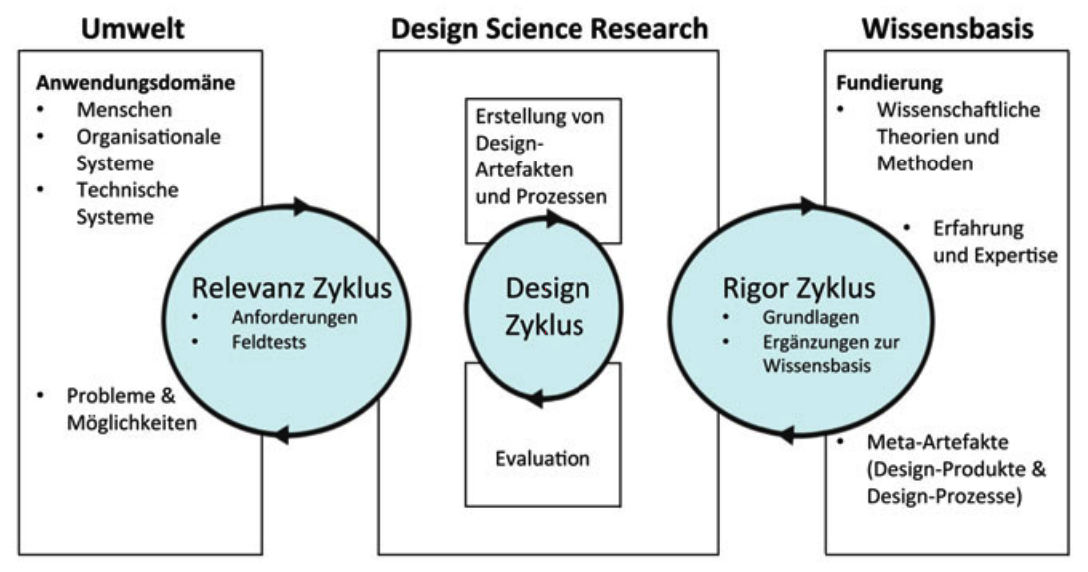
\includegraphics[width=0.70\linewidth]{pictures/three-cycles-design-science}
	\caption[Die drei Design Science Zyklen nach Hevner]{Die drei Design Science Zyklen nach \citet{Hevner2010}}
	\label{fig:three-cycles-design-science}
\end{figure}

Im Sinne des Relevanz Zyklus \citep[siehe auch][]{Simon1996} soll eine Betrachtung der bisherigen Supply Chain Systeme und der Wertschöpfungskette inklusive ihrer einzelnen Geschäftsprozesse aus technischer Sicht erfolgen. Als Ergebnis dieser Betrachtung sollen Anforderungen an das Artefakt identifiziert werden. Anschließend wird durch den Rigor Zyklus eine wisschenschaftliche Basis erarbeitet, um bereits vorhandene Erkenntnisse in die Arbeit einfließen zu lassen. Durch den Rigor Zyklus soll sichergestellt werden, dass das Artefakt eine Innovation darstellt und nicht bereits erforschte Resultate repliziert werden \citep{Hevner2010}. Innerhalb des Design Zyklus soll ein möglicher System Entwurf zur Lösung der Probleme aus Abschnitt \ref{Problemstellung} erarbeitet werden. Dieser System Entwurf wird als Prototyp implementiert und anschließend einer Evaluation durch Experteninterviews \citep[siehe auch][]{Wilde2007} unterzogen.

\newpage
